% Created by tikzDevice version 0.5.2 on 2011-03-14 15:14:44
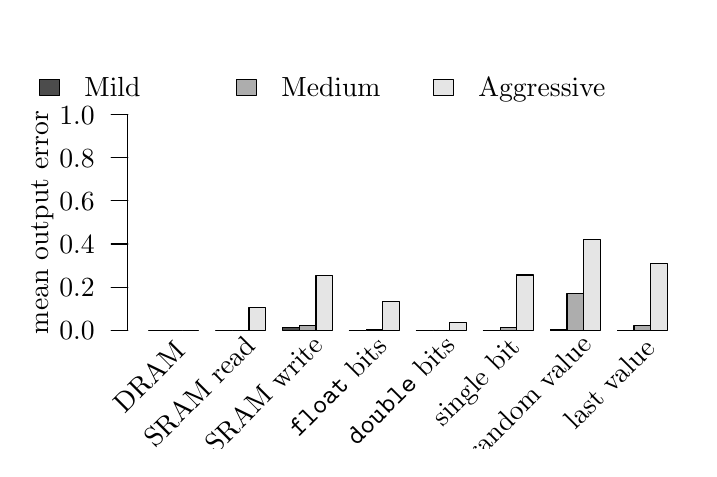
\begin{tikzpicture}[x=1pt,y=1pt]
\draw[color=white,opacity=0] (0,0) rectangle (238.49,151.77);
\begin{scope}
\path[clip] (  0.00,  0.00) rectangle (238.49,151.77);
\definecolor[named]{drawColor}{rgb}{0.18,0.00,0.42}
\definecolor[named]{fillColor}{rgb}{0.45,0.45,0.18}
\definecolor[named]{drawColor}{rgb}{0.00,0.00,0.00}
\definecolor[named]{fillColor}{rgb}{0.30,0.30,0.30}

\draw[color=drawColor,line cap=round,line join=round,fill=fillColor,] ( 43.50, 42.60) rectangle ( 49.55, 42.60);
\definecolor[named]{fillColor}{rgb}{0.68,0.68,0.68}

\draw[color=drawColor,line cap=round,line join=round,fill=fillColor,] ( 49.55, 42.60) rectangle ( 55.60, 42.60);
\definecolor[named]{fillColor}{rgb}{0.90,0.90,0.90}

\draw[color=drawColor,line cap=round,line join=round,fill=fillColor,] ( 55.60, 42.60) rectangle ( 61.64, 42.63);
\definecolor[named]{fillColor}{rgb}{0.30,0.30,0.30}

\draw[color=drawColor,line cap=round,line join=round,fill=fillColor,] ( 67.69, 42.60) rectangle ( 73.74, 42.60);
\definecolor[named]{fillColor}{rgb}{0.68,0.68,0.68}

\draw[color=drawColor,line cap=round,line join=round,fill=fillColor,] ( 73.74, 42.60) rectangle ( 79.79, 42.69);
\definecolor[named]{fillColor}{rgb}{0.90,0.90,0.90}

\draw[color=drawColor,line cap=round,line join=round,fill=fillColor,] ( 79.79, 42.60) rectangle ( 85.84, 50.97);
\definecolor[named]{fillColor}{rgb}{0.30,0.30,0.30}

\draw[color=drawColor,line cap=round,line join=round,fill=fillColor,] ( 91.88, 42.60) rectangle ( 97.93, 43.62);
\definecolor[named]{fillColor}{rgb}{0.68,0.68,0.68}

\draw[color=drawColor,line cap=round,line join=round,fill=fillColor,] ( 97.93, 42.60) rectangle (103.98, 44.43);
\definecolor[named]{fillColor}{rgb}{0.90,0.90,0.90}

\draw[color=drawColor,line cap=round,line join=round,fill=fillColor,] (103.98, 42.60) rectangle (110.03, 62.48);
\definecolor[named]{fillColor}{rgb}{0.30,0.30,0.30}

\draw[color=drawColor,line cap=round,line join=round,fill=fillColor,] (116.08, 42.60) rectangle (122.13, 42.60);
\definecolor[named]{fillColor}{rgb}{0.68,0.68,0.68}

\draw[color=drawColor,line cap=round,line join=round,fill=fillColor,] (122.13, 42.60) rectangle (128.17, 42.86);
\definecolor[named]{fillColor}{rgb}{0.90,0.90,0.90}

\draw[color=drawColor,line cap=round,line join=round,fill=fillColor,] (128.17, 42.60) rectangle (134.22, 53.02);
\definecolor[named]{fillColor}{rgb}{0.30,0.30,0.30}

\draw[color=drawColor,line cap=round,line join=round,fill=fillColor,] (140.27, 42.60) rectangle (146.32, 42.60);
\definecolor[named]{fillColor}{rgb}{0.68,0.68,0.68}

\draw[color=drawColor,line cap=round,line join=round,fill=fillColor,] (146.32, 42.60) rectangle (152.37, 42.62);
\definecolor[named]{fillColor}{rgb}{0.90,0.90,0.90}

\draw[color=drawColor,line cap=round,line join=round,fill=fillColor,] (152.37, 42.60) rectangle (158.41, 45.51);
\definecolor[named]{fillColor}{rgb}{0.30,0.30,0.30}

\draw[color=drawColor,line cap=round,line join=round,fill=fillColor,] (164.46, 42.60) rectangle (170.51, 42.60);
\definecolor[named]{fillColor}{rgb}{0.68,0.68,0.68}

\draw[color=drawColor,line cap=round,line join=round,fill=fillColor,] (170.51, 42.60) rectangle (176.56, 43.62);
\definecolor[named]{fillColor}{rgb}{0.90,0.90,0.90}

\draw[color=drawColor,line cap=round,line join=round,fill=fillColor,] (176.56, 42.60) rectangle (182.61, 62.61);
\definecolor[named]{fillColor}{rgb}{0.30,0.30,0.30}

\draw[color=drawColor,line cap=round,line join=round,fill=fillColor,] (188.65, 42.60) rectangle (194.70, 42.88);
\definecolor[named]{fillColor}{rgb}{0.68,0.68,0.68}

\draw[color=drawColor,line cap=round,line join=round,fill=fillColor,] (194.70, 42.60) rectangle (200.75, 55.92);
\definecolor[named]{fillColor}{rgb}{0.90,0.90,0.90}

\draw[color=drawColor,line cap=round,line join=round,fill=fillColor,] (200.75, 42.60) rectangle (206.80, 75.42);
\definecolor[named]{fillColor}{rgb}{0.30,0.30,0.30}

\draw[color=drawColor,line cap=round,line join=round,fill=fillColor,] (212.85, 42.60) rectangle (218.90, 42.64);
\definecolor[named]{fillColor}{rgb}{0.68,0.68,0.68}

\draw[color=drawColor,line cap=round,line join=round,fill=fillColor,] (218.90, 42.60) rectangle (224.94, 44.32);
\definecolor[named]{fillColor}{rgb}{0.90,0.90,0.90}

\draw[color=drawColor,line cap=round,line join=round,fill=fillColor,] (224.94, 42.60) rectangle (230.99, 66.89);
\end{scope}
\begin{scope}
\path[clip] (  0.00,  0.00) rectangle (238.49,151.77);
\definecolor[named]{drawColor}{rgb}{0.18,0.00,0.42}
\definecolor[named]{fillColor}{rgb}{0.45,0.45,0.18}
\definecolor[named]{drawColor}{rgb}{0.00,0.00,0.00}

\draw[color=drawColor,line cap=round,line join=round,fill opacity=0.00,] ( 36.00, 42.60) -- ( 36.00,120.57);

\draw[color=drawColor,line cap=round,line join=round,fill opacity=0.00,] ( 36.00, 42.60) -- ( 30.00, 42.60);

\draw[color=drawColor,line cap=round,line join=round,fill opacity=0.00,] ( 36.00, 58.19) -- ( 30.00, 58.19);

\draw[color=drawColor,line cap=round,line join=round,fill opacity=0.00,] ( 36.00, 73.79) -- ( 30.00, 73.79);

\draw[color=drawColor,line cap=round,line join=round,fill opacity=0.00,] ( 36.00, 89.38) -- ( 30.00, 89.38);

\draw[color=drawColor,line cap=round,line join=round,fill opacity=0.00,] ( 36.00,104.97) -- ( 30.00,104.97);

\draw[color=drawColor,line cap=round,line join=round,fill opacity=0.00,] ( 36.00,120.57) -- ( 30.00,120.57);

\node[color=drawColor,anchor=base east,inner sep=0pt, outer sep=0pt, scale=  1.00] at ( 24.00, 39.16) {0.0%
};

\node[color=drawColor,anchor=base east,inner sep=0pt, outer sep=0pt, scale=  1.00] at ( 24.00, 54.75) {0.2%
};

\node[color=drawColor,anchor=base east,inner sep=0pt, outer sep=0pt, scale=  1.00] at ( 24.00, 70.34) {0.4%
};

\node[color=drawColor,anchor=base east,inner sep=0pt, outer sep=0pt, scale=  1.00] at ( 24.00, 85.94) {0.6%
};

\node[color=drawColor,anchor=base east,inner sep=0pt, outer sep=0pt, scale=  1.00] at ( 24.00,101.53) {0.8%
};

\node[color=drawColor,anchor=base east,inner sep=0pt, outer sep=0pt, scale=  1.00] at ( 24.00,117.12) {1.0%
};

\node[rotate= 90.00,color=drawColor,anchor=base,inner sep=0pt, outer sep=0pt, scale=  1.00] at (  7.20, 81.58) {mean output error%
};
\end{scope}
\begin{scope}
\path[clip] (  0.00,  0.00) rectangle (238.49,151.77);
\definecolor[named]{drawColor}{rgb}{0.18,0.00,0.42}
\definecolor[named]{fillColor}{rgb}{0.45,0.45,0.18}
\definecolor[named]{drawColor}{rgb}{0.00,0.00,0.00}
\definecolor[named]{fillColor}{rgb}{0.30,0.30,0.30}

\draw[color=drawColor,line cap=round,line join=round,fill=fillColor,] (  4.11,133.40) rectangle ( 11.31,127.40);
\definecolor[named]{fillColor}{rgb}{0.68,0.68,0.68}

\draw[color=drawColor,line cap=round,line join=round,fill=fillColor,] ( 75.28,133.40) rectangle ( 82.48,127.40);
\definecolor[named]{fillColor}{rgb}{0.90,0.90,0.90}

\draw[color=drawColor,line cap=round,line join=round,fill=fillColor,] (146.44,133.40) rectangle (153.64,127.40);

\node[color=drawColor,anchor=base west,inner sep=0pt, outer sep=0pt, scale=  1.00] at ( 20.31,126.95) {Mild%
};

\node[color=drawColor,anchor=base west,inner sep=0pt, outer sep=0pt, scale=  1.00] at ( 91.48,126.95) {Medium%
};

\node[color=drawColor,anchor=base west,inner sep=0pt, outer sep=0pt, scale=  1.00] at (162.64,126.95) {Aggressive%
};

\node[rotate= 45.00,color=drawColor,anchor=base east,inner sep=0pt, outer sep=0pt, scale=  1.00] at ( 57.25, 34.61) {DRAM%
};

\node[rotate= 45.00,color=drawColor,anchor=base east,inner sep=0pt, outer sep=0pt, scale=  1.00] at ( 82.52, 36.38) {SRAM read%
};

\node[rotate= 45.00,color=drawColor,anchor=base east,inner sep=0pt, outer sep=0pt, scale=  1.00] at (106.95, 36.61) {SRAM write%
};

\node[rotate= 45.00,color=drawColor,anchor=base east,inner sep=0pt, outer sep=0pt, scale=  1.00] at (130.15, 36.27) {\texttt{float} bits%
};

\node[rotate= 45.00,color=drawColor,anchor=base east,inner sep=0pt, outer sep=0pt, scale=  1.00] at (154.71, 36.64) {\texttt{double} bits%
};

\node[rotate= 45.00,color=drawColor,anchor=base east,inner sep=0pt, outer sep=0pt, scale=  1.00] at (178.11, 35.89) {single bit%
};

\node[rotate= 45.00,color=drawColor,anchor=base east,inner sep=0pt, outer sep=0pt, scale=  1.00] at (204.00, 36.90) {random value%
};

\node[rotate= 45.00,color=drawColor,anchor=base east,inner sep=0pt, outer sep=0pt, scale=  1.00] at (226.94, 35.64) {last value%
};
\end{scope}
\end{tikzpicture}
